In diesem Kapitel wird die mechanische Konstruktion des Rollstuhl-Prototyps sowie die 
Auswahl geeigneter Antriebssysteme beschrieben. Zunächst wird die Struktur der drehbaren 
und hebbaren Plattform erläutert, die präzise Rotations-, Hebe- und Kippbewegungen des 
Rollstuhls ermöglicht. Anschließend wird auf die Funktionsweise der eingesetzten Wagenheber 
und deren koordinierte Steuerung eingegangen. Im weiteren Verlauf wird die Entscheidung für 
Schrittmotoren gegenüber hydraulischen Antrieben begründet, wobei Aspekte wie Präzision, 
Wiederholgenauigkeit, Flexibilität und Wartungsaufwand betrachtet werden. Das Kapitel 
vermittelt somit sowohl die konzeptionellen Überlegungen als auch die technischen 
Grundlagen, die die Beweglichkeit und Justierbarkeit des Rollstuhls im Prototypen 
sicherstellen.

\section{Aufbau des Prototyps}
\setauthor{Elisa Kaltenberger}

Der Prototyp ist so konstruiert, dass er sowohl präzise Rotationsbewegungen als auch 
kontrollierte Hebe- und Kippbewegungen des Rollstuhls ermöglicht. Die Konstruktion besteht 
aus zwei Platten, die in übereinander angeordneter Form miteinander verbunden sind. Die 
untere Platte befindet sich in einer stabilen und unbeweglichen Position und konstituiert 
die tragende Basis des Systems. Auf dieser befindet sich eine zweite Platte, die drehbar 
ausgeführt ist. Die Bewegung der oberen Platte wird durch ein Antriebsrad und einen 
Schrittmotor initiiert. Der Schrittmotor gestattet aufgrund seiner schrittweisen Bewegung 
eine exakte, fein dosierbare und wiederholgenaue Drehung. Die vorliegende Konstruktion 
ermöglicht eine millimetergenaue Einstellung der Ausrichtung des Rollstuhls. 

Auf der rotierenden oberen Platte sind drei Wagenheber montiert, die ausschließlich 
für das Heben und Kippen des Rollstuhls, der auf ihnen platziert wird. Zwei der 
Wagenheber sind links und rechts an den Seiten der Platte befestigt, sodass sie direkt 
unter den großen Rädern des Rollstuhls sind. Es obliegt den zuvor genannten Instanzen 
sowohl die Stabilisierung als auch die Hauptarbeit des Hebens. Die seitlichen Wagenheber 
können synchron betrieben werden, um den Rollstuhl gleichmäßig anzuheben, oder einzeln 
angesprochen werden, um eine einsteige Hubbewegung zu ermöglichen. Die asynchrone
Bestätigung des Rollstuhls erlaubt eine gezielte Kippfunktion, bei der der Rollstuhl 
kontrolliert auf einer Seite angehoben wird. In der Folge können Neigungen erzielt oder
bestimmte Positionen erreicht werden, die bei einem symmetrischen Anheben nicht möglich 
wären.

Der dritte Wagenheber ist im vorderen Bereich der drehbaren Platte positioniert und trägt 
ebenfalls aktiv zum Heben und Kippen des Rollstuhls bei. Im Gegensatz zu dem zuvor 
beschriebenen Wagenheber, der lediglich als Stütze dient, ist dieser vordere Wagenheber 
mit einer Funktion ausgestattet, die es ihm ermöglicht, den Rollstuhl eigenständig 
anzuheben und zu kippen. Aufgrund seiner Positionierung ermöglicht er eine kontrollierte 
Vorneigung oder eine kombinierte Kippbewegung in Verbindung mit einem der seitlichen 
Wagenheber. In der Konsequenz manifestiert sich ein System, dessen Funktionalität die 
Adjustierung des Rollstuhls in nahezu jede gewünschte Neigung ermöglicht, unabhängig davon, 
ob eine einseitige, vordere oder kombinierte Kippfunktion erforderlich ist.

Die drei Wagenheber bilden in Kombination ein flexibles Dreipunkt-Stütz- und Hebesystem, 
das sowohl vertikale Bewegungen als auch gezielte Kippvorgänge sicher und stabil ausführen 
kann. Die Wagenheber ermöglichen einen Höhen- und Neigungsverstellung des Rollstuhls, während 
die Plattform selbst eine konstante Bodenhaftung aufweist. Es sei darauf hingewiesen, dass 
der Schrittmotor erst nach der gewünschten Hebe- oder Kippbewegung die präzise rotatorische 
Ausrichtung übernimmt- In diesem Prozess werden der Wagenheber und der Rollstuhl vollständig 
mit der drehbaren Platte vollständig mit der drehbaren Platte mitgeführt.

\section{Bauungsprozess Hardware Prototyp}
\setauthor{Elisa Kaltenberger}
in diesem kapitel geht es um....

\begin{figure}
    \centering
    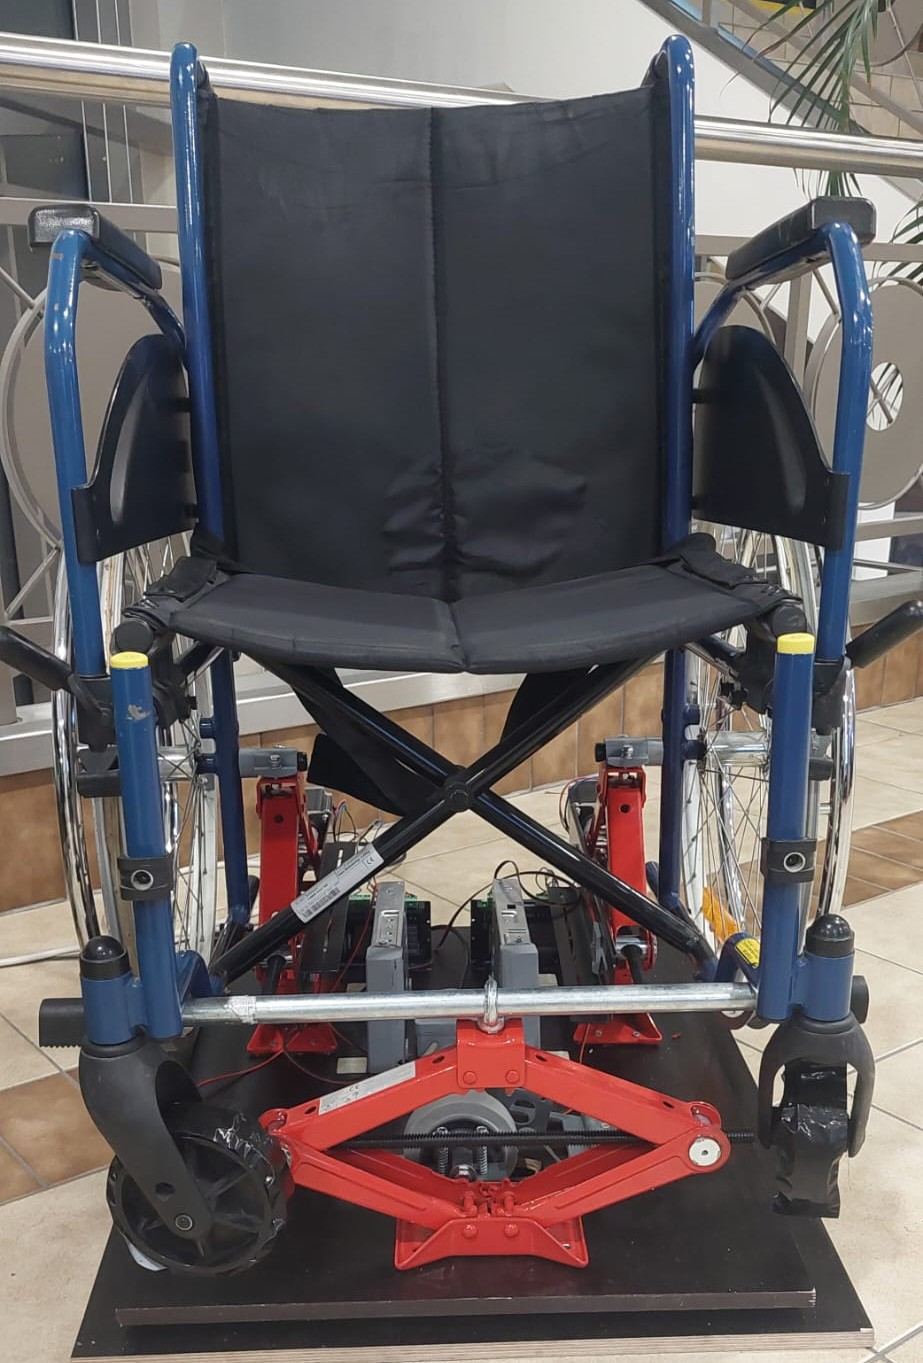
\includegraphics[scale=0.3]{pics/prototyp-ende.jpg}
    \caption{Prototyp Ende 21. November}
    \label{fig:prototyp-ende}
\end{figure}


\subsection{Motorenfindung: Schrittmotoren vs. Hydraulik}
\setauthor{Elisa Kaltenberger}

Hydrauliksysteme arbeiten mit Flüssigkeiten unter Druck, um signifikante Kräfte zu generieren. 
Die Verdrängung von Hydrauliköl durch einen Kolben ermöglicht die Erzeugung eines hohen Drucks, 
der die Bewegung schwerer Lasten oder präziser mechanischer Bewegung ermöglicht.

Derartige Systeme erweisen sich als vorteilhaft, wenn es darum geht, große Kräfte, Drehmomente oder 
schwere Lasten zu bewegen. Dies ist beispielsweise in Baumaschinen, Hebebühnen oder bei Pressen der 
Fall.

Allerdings sind hydraulische Anlagen in der Regel durch eine komplexe Konstruktion charakterisiert, 
die Zylinder, Pumpen und eine Ölfüllung umfasst. Dies impliziert hohe Wartungsaufwendungen, eine 
aufwändige Installation sowie eine eingeschränkte Flexibilität, insbesondere in Bezug auf feinfühlige 
oder kontrollierte Bewegungen.

Sofern die betreffende Anwendung keine extrem schweren Lasten bewegt, sondern eher präzise, kontrollierte 
und wiederholbare Bewegung erfordert, ist eine Hydraulik-Lösung oft zu aufwändig.

Ein Schrittmotor hingegen ist ein bürstenloser Gleichstrommotor, dessen Rotationsbewegung nicht 
kontinuierlich, sondern in vorgegebenen und gleichmäßigen Schritten erfolgt.

Die Position lässt sich dadurch mit hoher Präzision, Reproduzierbarkeit und ohne zusätzliche Rückführung 
bestimmen. Dies ist vorteilhaft, wenn eine exakte Positionierung oder punktgenaue Steuerung erforderlich ist.

Die Realisierung von sehr feinen Schritten ist durch den Einsatz von Mikroschritt-Antrieben möglich, 
wodurch die Bewegungen nahezu glatt und servo-ähnlich wirken, ohne dass ein geschlossener Regelkreis 
erforderlich ist.

Darüber hinaus zeichnen sich Schrittmotoren im Vergleich zu hydraulischen Systemen durch eine kompakte 
Bauweise, ein geringes Gewicht, eine einfache Handhabung und Wartung aus. Es besteht keine Notwendigkeit 
für eine Ölversorgung, hydraulische Leitungen oder Zylinder, was Platz, Aufwand und potenzielle Fehlerquellen 
reduziert. 

Zusätzlich sind Schrittmotoren insbesondere dann sinnvoll, wenn die Anwendung häufige, gleichförmige oder 
wiederholbare Bewegungen erfordert, wie sie beispielsweise bei der Indexierung, Positionierung oder 
automatisierten Abläufen auftreten, und die Last gleichmäßig und vorhersehbar ist.

\subsection{Bauprozess}
Nachdem entschieden worden war, welche Antriebsart verwendet werden sollte, wurden die Motoren bestellt. 
Während der Lieferzeit machte man sich Gedanken darüber, wie die Konstruktion des Prototyps aussehen könnte. 
Die Überlegung war, auf einer Holzplatte eine zweite Platte zu montieren, die mithilfe von Rollen auf der 
unteren Platte beweglich ist. An der Unterseite dieser oberen, horizontal beweglichen Platte wurden kleine 
Rollen befestigt, die die horizontale Bewegung ermöglichen.

Zusätzlich wurde in die obere Holzplatte ein längliches Loch gefräst, sodass ein größeres Gummirad 
darin Platz findet. Dieses Rad ermöglicht die eigentliche horizontale Drehbewegung. Das Gummirad wurde 
anschließend mithilfe eines selbst gefertigten 3D-gedruckten Bauteils auf der oberen Platte befestigt 
(siehe Abb. 5: Befestigung des Gummirads). 

Das 3D-Teil wurde in KiCad konstruiert und in der Schule im Keller gedruckt. Es wurde dem Filament 
ABS gedruckt. Es wurde Acrylnitril-Butadien-Styrol (ABS) gewählt, denn es zeichnet sich durch eine 
hohe Steifigkeit, 
Zähigkeit und Festigkeit aus. Das Material zeichnet sich durch eine hohe Schlag- und Kratzfestigkeit 
aus und weist eine hohe Resilienz gegenüber mechanischen Belastungen auf. Zudem ist ABS beständig 
gegenüber Ölen, Fetten und vielen Chemikalien. Es weist eine gute Temperaturbeständigkeit auf und 
bleibt auch bei höheren Temperaturen formstabil. Außerdem lässt sich ABS vielseitig verarbeiten und 
gut nachbearbeiten, beispielsweise durch Schleifen oder Lackieren.
(Quelle 11)

\begin{figure}
    \centering
    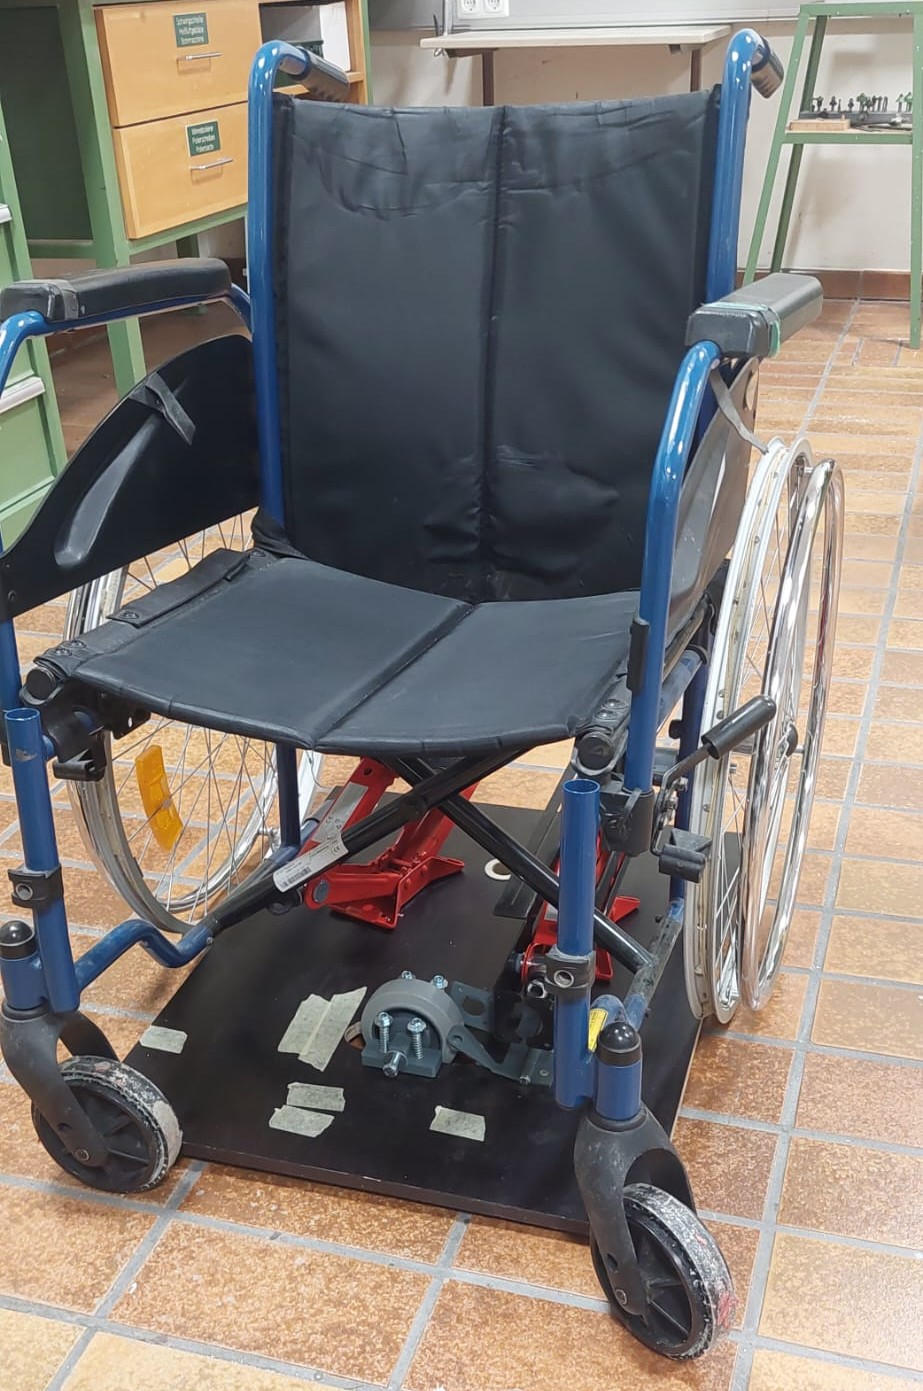
\includegraphics[scale=0.3]{pics/prototyp-zwischenstand.jpg}
    \caption{Prototyp Zwischnstand 13. November}
    \label{fig:prototyp-zwischenstand}
\end{figure}

Nachdem alles angeschraubt wurde, wurden die Wagenheber provisorisch positioniert, um einen ersten 
Eindruck von den Prototypen zu gewinnen, siehe Abb. \ref{fig:prototyp-zwischenstand}.

\subsection{Fertigung der Platine}
\setauthor{Elisa Kaltenberger}
Die Fertigung der Platine stellt einen zentralen Bestandteil des gesamten Entwicklungsprozesses dar 
und bildet die Grundlage für die zuverlässige Funktion der elektronischen Schaltung. Von der ersten 
Konzeption über die Layoutgestaltung bis hin zur eigentlichen Herstellung erfordert dieser Prozess 
ein präzises und systematisches Vorgehen. Sowohl die sorgfältige Planung mit geeigneten 
Entwicklungswerkzeugen als auch die fachgerechte Durchführung der einzelnen Fertigungsschritte 
tragen maßgeblich zur Qualität, Betriebssicherheit und Langlebigkeit der Leiterplatte bei.

Im Folgenden werden zunächst die Entwurfsphase der Leiterplatte sowie anschließend der technische 
Aufbau und die einzelnen Schritte des Herstellungsprozesses detailliert beschrieben.

\subsection{Layout in KiCad}
\setauthor{Elisa Kaltenberger}
Vor Beginn des eigentlichen Herstellungsprozesses wurde die Leiterplatte mithilfe von KiCad 
vollständig geplant und vorbereitet. Im ersten Schritt erfolgte die Erstellung eines detaillierten 
Schaltplans. Darin wurden sämtliche elektronischen Komponenten, einschließlich ihrer elektrischen 
Verbindungen, systematisch erfasst und eindeutig definiert. Der Fokus lag dabei auf einer klar 
strukturierten Darstellung, einer logisch aufgebauten Verschaltung sowie einer durchdachten Auswahl 
geeigneter Bauteile im Hinblick auf Funktionalität, Verfügbarkeit und elektrische Belastbarkeit.

Nach der sorgfältigen Überprüfung und Finalisierung des Schaltplans Abb.\ref{fig:schaltplan} wurde das Projekt in den 
Platinen-Editor von KiCad übertragen. Dort begann die konkrete Layoutgestaltung der Leiterplatte. 
Zunächst wurden alle Bauteile unter Berücksichtigung funktionaler Zusammenhänge sinnvoll auf der 
Leiterplatte positioniert. Ziel war es, kurze Signalwege zu ermöglichen, kritische Leitungen zu 
trennen und eine möglichst übersichtliche Anordnung zu schaffen. Auch mechanische Aspekte, wie 
Befestigungspunkte oder spätere Einbaumöglichkeiten, wurden dabei berücksichtigt.

\begin{figure}
    \centering
    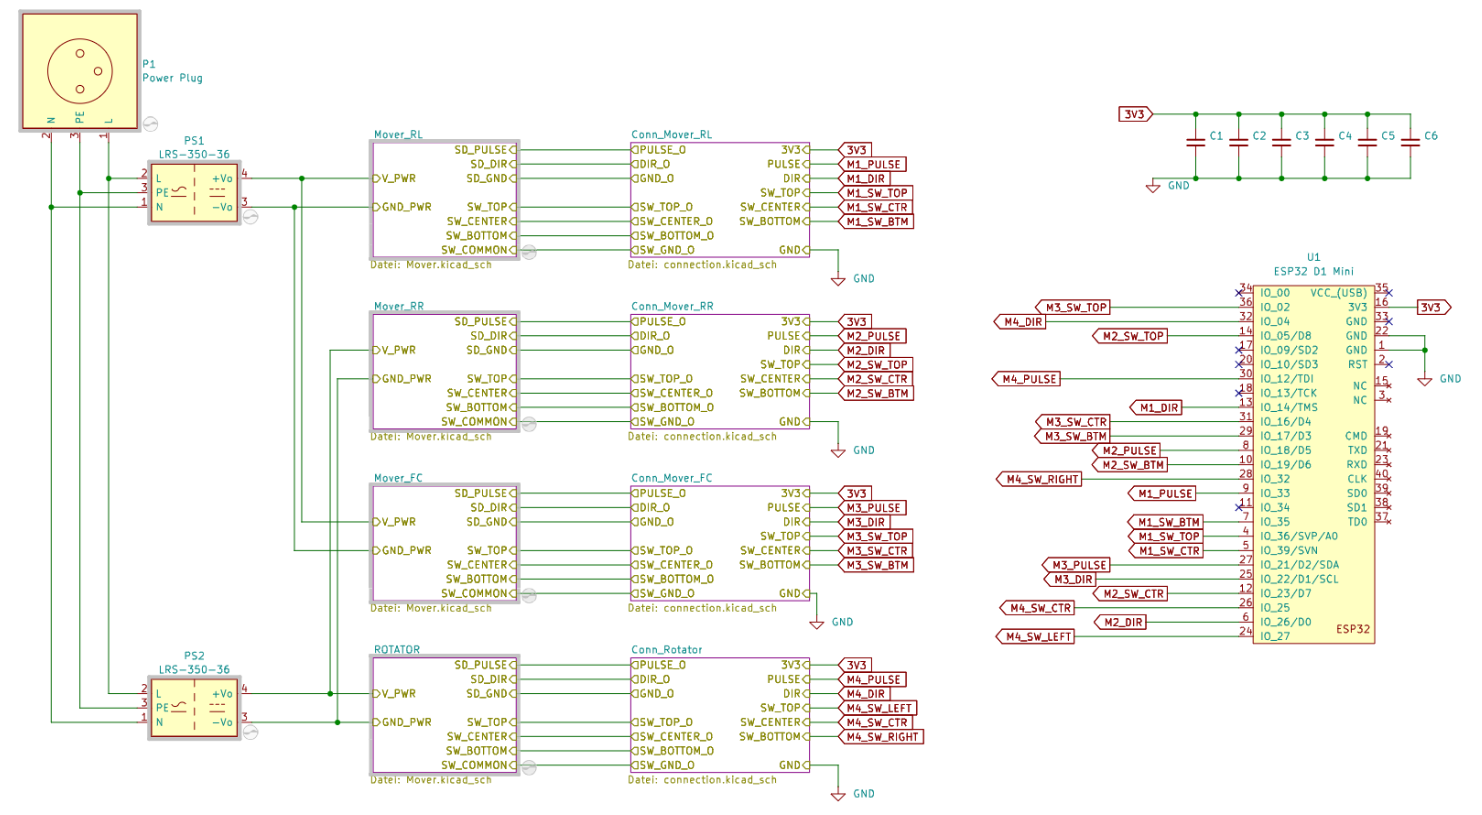
\includegraphics[scale=0.5]{pics/Schaltplan.png}
    \caption{Schaltplan der Platine}
    \label{fig:schaltplan}
\end{figure}

Im nächsten Schritt erfolgte das Routing der Leiterbahnen. Hierbei wurde darauf geachtet, 
Signalstörungen zu minimieren, Kreuzungen möglichst zu vermeiden und eine saubere, nachvollziehbare 
Leitungsführung zu gewährleisten. Versorgungsleitungen wurden entsprechend dimensioniert, während 
empfindliche Signalleitungen mit besonderer Sorgfalt behandelt wurden. Zusätzlich wurden sämtliche 
Designregeln, wie Mindestabstände zwischen Leiterbahnen, geeignete Leiterbahnbreiten sowie Vorgaben 
für Durchkontaktierungen, konsequent eingehalten. Abschließend wurde das Layout nochmals überprüft, 
um mögliche Fehler frühzeitig zu erkennen und eine reibungslose Fertigung der Platine sicherzustellen.

\subsection{Platinenherstellung}
\setauthor{Elisa Kaltenberger}
Bei der Herstellung von Leiterplatten kommt dem konstruktiven Aufbau sowie der präzisen Abstimmung 
der einzelnen Fertigungsschritte eine entscheidende Bedeutung zu. Diesbezüglich sind insbesondere die 
spätere Funktionalität, Lebensdauer und Betriebssicherheit zu berücksichtigen. Bereits geringfügige 
Abweichungen im Prozess können die elektrische Leitfähigkeit, die mechanische Stabilität oder die 
Lötqualität erheblich beeinflussen.

Eine typische Leiterplatte besteht im Wesentlichen aus mehreren aufeinander abgestimmten Schichten. 
Die Grundlage bildet das Basismaterial, häufig ein glasfaserverstärktes Epoxidharz. Dieses dient als 
mechanische Trägerstruktur und sorgt gleichzeitig für die notwendige elektrische Isolation zwischen 
den leitenden Strukturen. Auf dieses Substrat wird eine dünne Kupferschicht aufgebracht beziehungsweise 
auflaminiert. Sie stellt das eigentliche leitfähige Material dar, aus dem später die Leiterbahnen, 
Masseflächen und Kontaktpads entstehen. Abschließend wird die Oberfläche mit einer lichtempfindlichen 
Fotolackschicht versehen. Diese fungiert als temporäre Schutz- und Maskierungsschicht, mit deren Hilfe 
das gewünschte Leiterbild präzise übertragen werden kann.

Der eigentliche Fertigungsprozess erfolgt in mehreren aufeinander abgestimmten Schritten. Zu Beginn des 
Verfahrens wird die mit Fotolack beschichtete Kupferfläche mittels UV-Licht belichtet. Hierbei wird eine 
Belichtungsvorlage verwendet, welche die späteren Leiterbahnen abbildet. An den belichteten Stellen erfolgt 
eine Aushärtung des Fotolacks, wodurch eine chemische Beständigkeit des Materials gewährleistet wird. Die 
unbelichteten Bereiche bleiben hingegen löslich.

Darauf folgt die Entwicklung der Platine in einer geeigneten Entwicklerlösung, die häufig auf Basis von 
Natronlauge basiert.  In diesem Schritt werden die nicht ausgehärteten Fotolackanteile entfernt, wodurch das 
darunterliegende Kupfer freigelegt wird. Das gewünschte Leiterbild wird dadurch erstmals sichtbar, da nur 
die durch den gehärteten Fotolack geschützten Bereiche erhalten bleiben.

Im darauffolgenden Ätzprozess wird das freiliegende, ungeschützte Kupfer unter Einsatz spezifischer Ätzmittel 
einer chemischen Reaktion unterzogen, die zu dessen Abtrag führt. Das Kupfer ist das einzige Element, das nach 
der Behandlung übrig bleibt und zuvor durch den gehärteten Fotolack geschützt wurde. Diese bilden nun die 
endgültigen Leiterbahnen der Schaltung. Je nach Aufbau der Platine können danach zusätzliche Arbeitsschritte 
wie das Bohren von Bauteil- und Durchkontaktierungslöchern erfolgen. Bei mehrlagigen Leiterplatten werden 
diese Bohrungen metallisiert, um elektrische Verbindungen zwischen verschiedenen Kupferschichten herzustellen.

Nach dem Ätzvorgang wird der verbliebene Fotolack im sogenannten Entschichtungsprozess vollständig entfernt. 
Die Kupferoberflächen werden gereinigt und gegebenenfalls chemisch nachbehandelt, um eine optimale 
Weiterverarbeitung zu gewährleisten. Im darauffolgenden Schritt wird die Lötstoppmaske aufgebracht. Diese 
Schutzschicht bedeckt nahezu die gesamte Leiterplatte und lässt lediglich die Lötpads frei. Sie schützt die 
Leiterbahnen vor Oxidation, verhindert ungewollte Lötbrücken und verbessert die elektrische sowie mechanische 
Zuverlässigkeit.

Nachdem alle Schritte der Platinenherstellung erfolgreich abgeschlossen wurden Abb. \ref{fig:platine}, 
wurden LEDS und Wiederstände auf der Platine verlötet. Es wurden LEDs und Widerstände verbaut, um die 
Funktionalität der Platine zu gewährleisten. Die LEDs dienen als visuelle Indikatoren für den Betriebszustand 
der Schaltung, während die Widerstände den Stromfluss regulieren und somit die Bauteile vor Überlastung 
schützen. Die sorgfältige Auswahl und Anordnung dieser Komponenten auf der Platine tragen maßgeblich zur 
Stabilität und Zuverlässigkeit der elektronischen Schaltung bei.
(Quelle 12 bis 16)

\begin{figure}
    \centering
    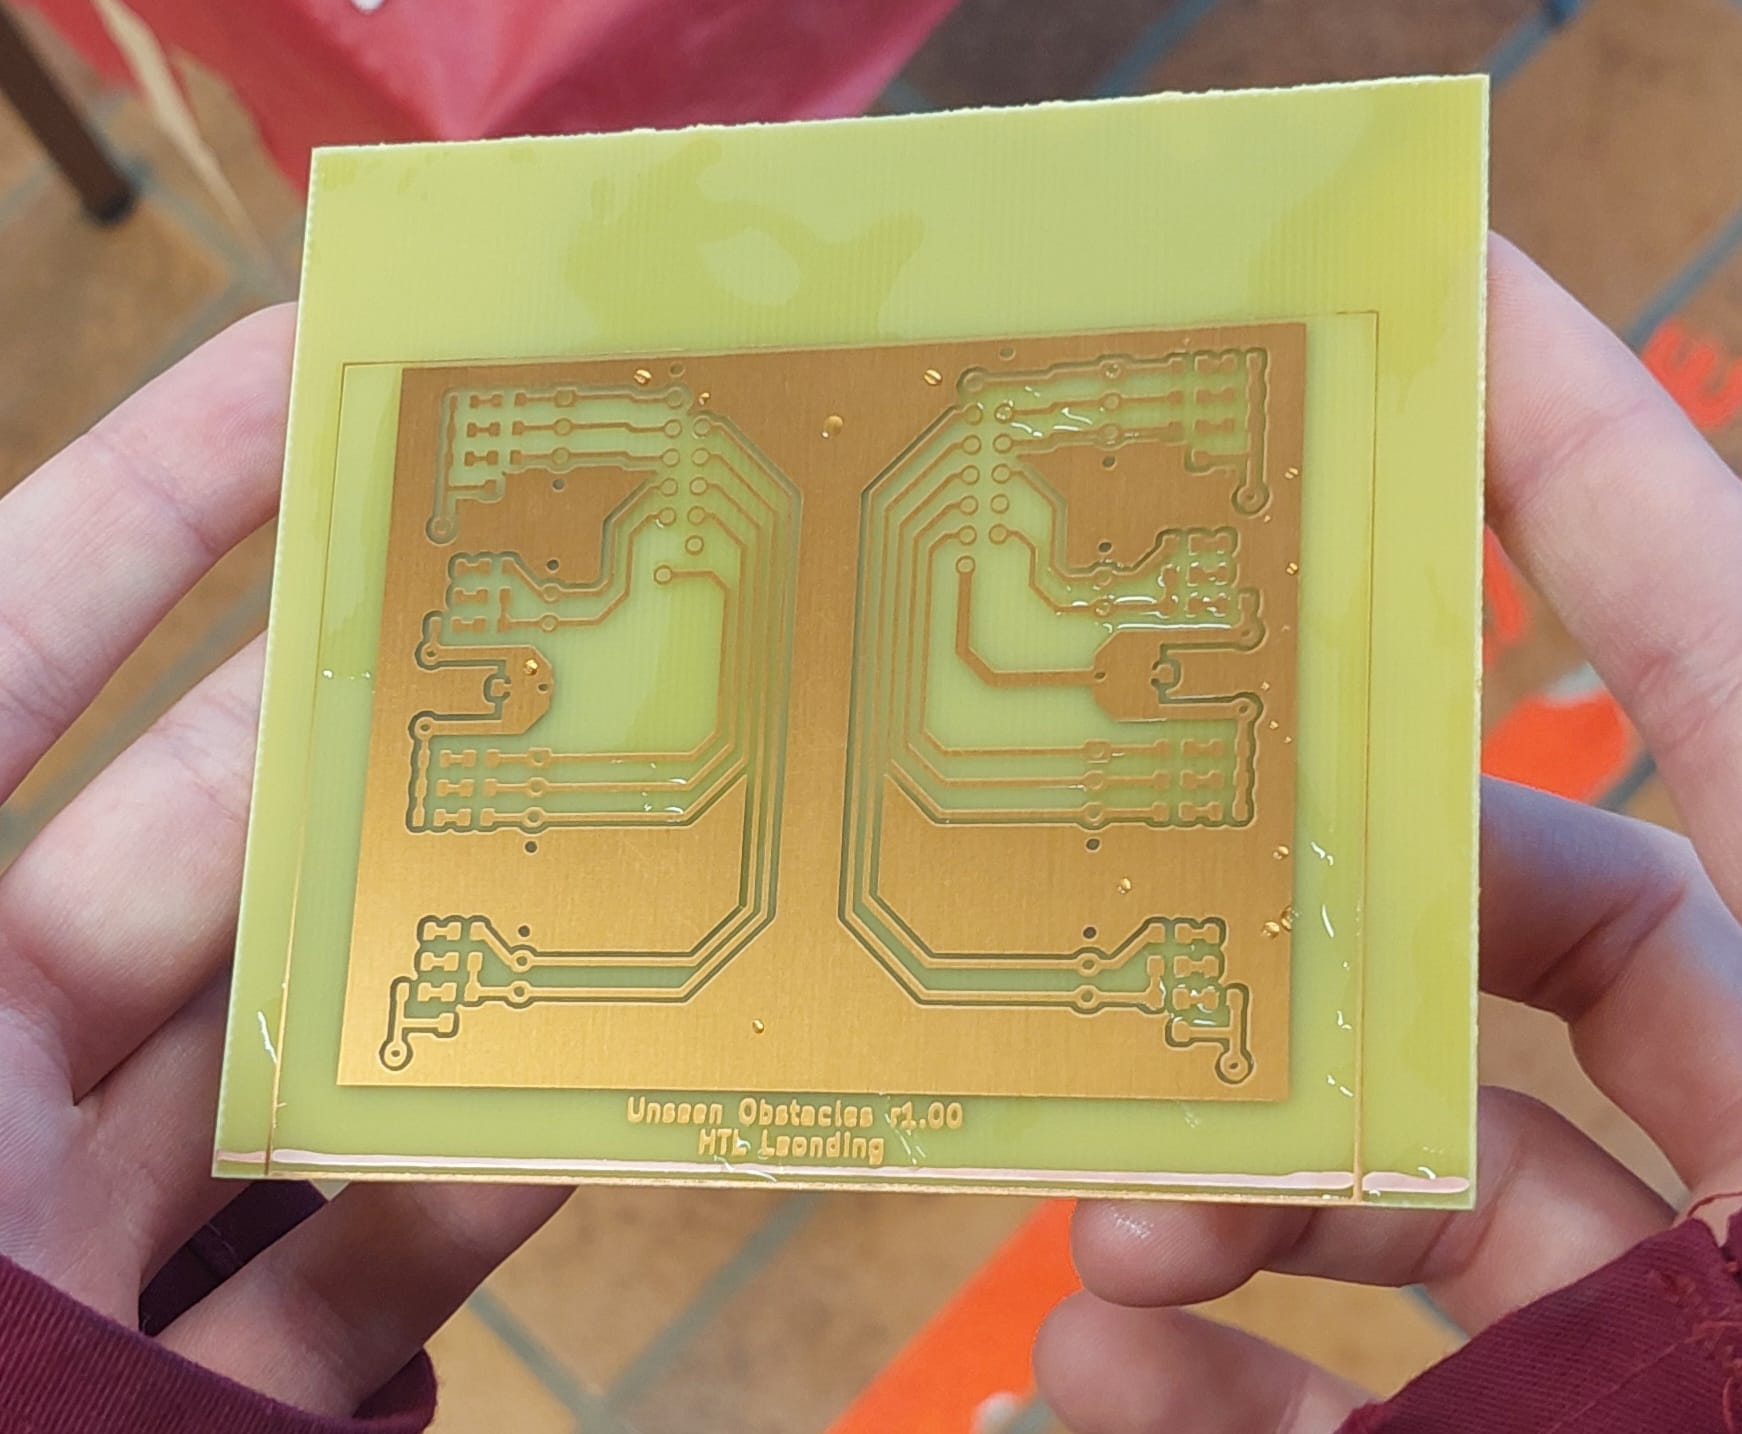
\includegraphics[scale=0.2]{pics/platine.jpg}
    \caption{Platine Prototyp}
    \label{fig:platine}
\end{figure}
